\section{Introduction}
\label{sec:introduction}

Frequency generators are electronic devices widely used in laboratories to generate electrical waves with the desired shapes. The most common waveforms used are sinusoidal, triangular, and square, but sometimes sinc, noise, and other less common waves are also used.
To generate an analog waveform with a digital circuit, different techniques are used, but each one is made of these blocks

\begin{itemize}
        
    \item \textbf{Human-Machine interface} \newline
    It is used to choose the waveform to be generated

    \item \textbf{Digital waveform generator} \newline
    It is the digital block that sends data to be converted into analog signals with the right timing specifications

    \item \textbf{Digital analog converter} \newline
    It is the component that converts the digital signals into analog signals
        
\end{itemize}

\noindent
The main blocks used to implement the function generator will now be briefly described.

\subsection{DDFS tecnique}

The DDFS tecnique also called \textbf{Direct Digital Frequency synthesis} is a type of digital electronic signal generator that read the data stored in a memory called LUT or \textbf{Look Up Table} to generate the samples for the desired signal.
\begin{center}
    \vspace*{1cm}
    \scalebox{0.79}{
        \begin{tikzpicture}
            \tikzset{one bit adder/.style={muxdemux,
                muxdemux def={Lh=4, NL=2, Rh=2, NR=1, NB=1, w=2.5,
                inset w=0.5, inset Lh=2, inset Rh=1.5}}}
                        
            \node[one bit adder, fill=cyan!30!white] (fa) at (6.53, 4) {\Large $\oplus$};
            \node[flipflop D, xscale=0.7, yscale=0.7, fill=cyan!30!white] at (9.784, 3.412){};
            \draw (7.5, 4) to[multiwire] (9, 4);
            \draw (10.568, 4) -| (11, 4) -| (11, 6.5) to[multiwire] (4.75, 6.5) -- (4.75, 4.84) -| (5.55, 4.84);
            \draw (5.55, 3.161) to[multiwire] (3, 3.161);
            \draw (9, 2.824) -| (8, 2) to[multiwire] (3, 2);
            \node[shape=rectangle, draw, line width=1pt, minimum width=1.965cm, minimum height=3.215cm, fill=cyan!30!white](N1) at (13, 4){} node[anchor=center] at (N1.text){$LUT$};
            \draw (11, 4) to[multiwire] (12, 4);
            \node[shape=rectangle, minimum width=0.8cm, minimum height=0.465cm] 
            at (2.625, 3.75) {};
        
            \node[
                shape=rectangle,
                minimum width=0.8cm,
                minimum height=0.465cm,
                align=center
            ] at (2.625, 3.2) {fw};
    
            \node[
                shape=rectangle,
                minimum width=0.8cm,
                minimum height=0.465cm,
                align=center
            ] at (2.625, 2.05) {clk};
        
        \end{tikzpicture}
    }
    \vspace*{1cm}        
\end{center}

\noindent
The DDFS signal generator is based on a counter called \textbf{phase accumulator}. \newline
The output of this counter is increased, at every positive edge of the clock signal, by the value stored in the variable \(f_w\), called \textbf{frequency word}. \newline
Then, the output of the counter is used as the address for a Look-Up Table memory that contains the samples of the signal to be generated.

\newpage

\subsubsection{Amplitude quantization}
The digital output value from the LUT is sent to an external \textbf{digital to analog converter}, and the number of bits used to store each sample of the wave determines the smallest amplitude swing that the wave can produce.\\
If we use a \textbf{C2 balanced representation} to generate the wave, the smallest output voltage swing is

\vspace*{0.25cm} 
\[
    min( \Delta V_{out} ) = \frac{V_{cc}}{2^N - 1}
\]
\vspace*{0.25cm} 

\noindent
where \(N\) is the number of bits for the signal samples and \(V_{cc}\) is the maximum output voltage of the DAC.

\subsubsection{Frequency quantization}
The samples are sent to the DAC at the clock frequency; indeed, at every positive edge of the clock, the flip-flop updates the output and the adder increases the input of the register for the next address value.  \\
The address does not increase by a unit amount, but depends on the value of \(f_w\); with this procedure, we can control the frequency of the output wave simply by adjusting the value of \(f_w\). \\
The output frequency of the wave is

\vspace*{0.25cm} 
\[
    f = f_{clk} \cdot \frac{f_{w}}{\texttt{LUT\_DIM}}
\]
\vspace*{0.25cm} 

\noindent
where \(f_{clk}\) is the clock frequency of the DDFS and \(LUT\_DIM\) is the number of samples stored in the LUT.
The problem is that increasing the value of \(f_w\) involves an increase in the output wave frequency, but a reduction in the number of samples used for the generation of the wave, which results in a stepped output signal.

\newpage

\subsubsection{LUT optimization}
Some types of waves have a quadrangular-symmetrical profile, meaning a periodic signal that, every quarter of its period, is reproduced by a vertical symmetry, and every half of its period by a horizontal symmetry.

\begin{center}

    \vspace*{0.5cm}
    \scalebox{0.9}{
        \begin{minipage}{0.45\textwidth}
            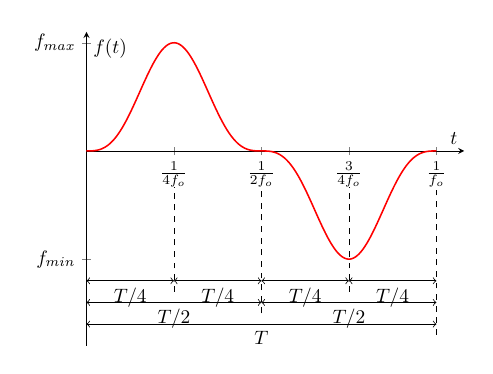
\begin{tikzpicture}[scale=0.7]
                \begin{axis}[
                    axis lines = middle,
                    xlabel = {$t$},
                    ylabel = {$f(t)$},
                    xmin = 0, xmax = 2*pi+0.5,
                    ymin = -1.8, ymax = 1.1,
                    samples = 200,
                    xtick = {pi/2, pi, 3*pi/2, 2*pi},
                    xticklabels = {$\frac{1}{4f_o}$, $\frac{1}{2f_o}$, $\frac{3}{4f_o}$, $\frac{1}{f_o}$},
                    ytick = {-1, 0, 1},
                    yticklabels = {$f_{min}$, 0, $f_{max}$}
                ]
                
                \addplot [red, thick, domain=0:2*pi] {sin(deg(x))^3};
                
                \draw[dashed] (axis cs:2*pi, -1.7) -- (axis cs:2*pi, -0.33);
                \draw[dashed] (axis cs:pi, -1.5) -- (axis cs:pi, -0.33);
                \draw[dashed] (axis cs:pi/2, -1.3) -- (axis cs:pi/2, -0.33);
                \draw[dashed] (axis cs:3*pi/2, -1.3) -- (axis cs:3*pi/2, -0.33);
                
                \draw[<->] (axis cs:0, -1.6) -- node[below] {$T$} (axis cs:2*pi, -1.6);
                \draw[<->] (axis cs:0, -1.4) -- node[below] {$T/2$} (axis cs:pi, -1.4);
                \draw[<->] (axis cs:pi, -1.4) -- node[below] {$T/2$} (axis cs:2*pi, -1.4);
                \draw[<->] (axis cs:0, -1.2) -- node[below] {$T/4$} (axis cs:pi/2, -1.2);
                \draw[<->] (axis cs:pi/2, -1.2) -- node[below] {$T/4$} (axis cs:pi, -1.2);
                \draw[<->] (axis cs:pi, -1.2) -- node[below] {$T/4$} (axis cs:3*pi/2, -1.2);
                \draw[<->] (axis cs:3*pi/2, -1.2) -- node[below] {$T/4$} (axis cs:2*pi, -1.2);
                
                \end{axis}
                
            \end{tikzpicture}
        \end{minipage}
        \hfill
        \begin{minipage}{0.45\textwidth}
            \scalebox{0.9}{
                \parbox{\linewidth}{
                    \textbf{Vertical symmetry:}
                    \[
                        \begin{aligned}
                            f\Bigl(\frac{T}{4}+t\Bigr) &= f\Bigl(\frac{T}{4}-t\Bigr) \quad t \in [0,T/2] \\
                            f\Bigl(\frac{3T}{4}+t\Bigr) &= f\Bigl(\frac{3T}{4}-t\Bigr) \quad t \in [T/2,T]
                        \end{aligned}
                    \]
                    
                    \textbf{Horizontal symmetry:}
                    \[
                        \begin{aligned}
                            f\Bigl(\frac{T}{2}+t\Bigr) &= -f\Bigl(\frac{T}{2}-t\Bigr) \quad t \in [0,T]
                        \end{aligned}
                    \]
                }
            }
        \end{minipage}
    }
    \vspace*{0.5cm} 

\end{center}

\noindent
For this type of wave, it is sufficient to store a quarter of the full period, and by reading the value of the phase accumulator, it can be determined whether vertical symmetry or horizontal symmetry needs to be applied.  \\
With this technique the dimension of the LUT can be reduced by a factor of 4. \\
To apply vertical symmetry, the LUT must be read from bottom to top, and to apply horizontal symmetry, the output signal must be inverted by changing its sign.  \\
Vertical symmetry should be applied during the second and fourth quarters of the period, while horizontal symmetry should be applied during the second half of the period. Therefore, if the LUT size is a power of two, the vertical symmetry signal can be \(y(MSB-1)\) and the horizontal symmetry signal \(y(MSB)\), where \(y(n)\) is the n-th output bit of the phase accumulator.
Using a C2 representation the \textbf{LUT optimization circuit} can be done as follows

\begin{center}
    \vspace*{1cm}
    \scalebox{0.79}{
        \begin{tikzpicture}
            \tikzset{one bit adder/.style={muxdemux,
                muxdemux def={Lh=4, NL=2, Rh=2, NR=1, NB=1, w=2.5,
                inset w=0.5, inset Lh=2, inset Rh=1.5}}}
            \tikzset{mux/.style={muxdemux,
                muxdemux def={Lh=4, NL=2, Rh=3,
                NB=1, w=2, square pins=1}}}
                        
            \node[one bit adder, fill=cyan!30!white] at (6.53, 4) {\Large $\oplus$};
            \node [mux, fill=red!30!white] (mux1) at (4, 3.16){MUX};
            \node [mux, fill=red!30!white] (mux2) at (18, 3.45){MUX};
            \node[flipflop D, xscale=0.7, yscale=0.7, fill=cyan!30!white] at (9.784, 3.412){};
            \draw (7.5, 4) to[multiwire] (9, 4);
            \draw (10.568, 4) -| (11, 4) -| (11, 6.5) to[multiwire] (4.75, 6.5) -- (4.75, 4.84) -| (5.55, 4.84);
            \draw (5.55, 3.161) to[multiwire] (4.835, 3.161);
            \draw (9, 2.824) -| (8, 0) -- (1, 0);
            \node[shape=rectangle, draw, line width=1pt, minimum width=1.965cm, minimum height=3.215cm, fill=cyan!30!white](N1) at (13, 4){} node[anchor=center] at (N1.text){$LUT$};
            \draw (11, 4) to[multiwire] (12, 4);
            \node[shape=rectangle, minimum width=0.8cm, minimum height=0.465cm] 
            at (2.625, 3.75) {};
            
            \node[ieeestd not port, rotate=0, scale=0.4, fill=red!30!white] (not1) at ($(mux1.lpin 2)+(-0.5,0)$) {};
            \node[ieeestd not port, rotate=0, scale=0.4, fill=red!30!white] (not2) at ($(mux2.lpin 2)+(-0.5,0)$) {};
            
            \node[
                shape=rectangle,
                minimum width=0.8cm,
                minimum height=0.465cm,
                align=center
            ] (fw) at ($(mux1.lpin 1) + (-2.5,0)$) {fw};

             \node[
                shape=rectangle,
                minimum width=0.8cm,
                minimum height=0.465cm,
                align=center
            ] (y1) at ($(mux1.bpin 1) + (0,-0.7)$) {y(MSB-1)};

            \draw (mux1.bpin 1) -- ($(mux1.bpin 1) + (0,-0.4)$);

            \node[
                shape=rectangle,
                minimum width=0.8cm,
                minimum height=0.465cm,
                align=center
            ] (y2) at ($(mux2.bpin 1) + (0,-0.7)$) {y(MSB)};
            
            \node[
                shape=rectangle,
                minimum width=0.8cm,
                minimum height=0.465cm,
                align=center
            ] (y2) at (9.85, 6.8) {y(MSB-2 .. 0)};

            \draw (mux2.bpin 1) -- ($(mux2.bpin 1) + (0,-0.4)$);
            
            \draw ($(mux1.lpin 1) + (-2.2,0)$) to[multiwire] (mux1.lpin 1);
            \draw (not1.in) -| ($(mux1.lpin 1) + (-1.7,0)$);
            \draw (not2.in) -| ($(mux2.lpin 1) + (-1.7,0)$);

            \draw (not1.out) -- (mux1.lpin 2);
            \draw (not2.out) -- (mux2.lpin 2);

            \draw (14, 4) to[multiwire] (15.5, 4);
            \draw (15.5, 4) to[multiwire] (mux2.lpin 1);
    
            \node[
                shape=rectangle,
                minimum width=0.8cm,
                minimum height=0.465cm,
                align=center
            ] at (0.65, 0.05) {clk};
        
        \end{tikzpicture}
    }
    \vspace*{1cm}
    
\end{center}


\newpage

\subsection{Parallel bus DAC}

The DAC, or \textbf{digital to analog converter}, is a device that takes a digital value as input and provides an analog output signal proportional to it. \\
The output voltage of the DAC can be calculated with the following formula


\vspace*{0.25cm} 
\[
    V_{out} = \frac{n}{2^N-1} \cdot V_{max}
\]
\vspace*{0.25cm} 

\noindent
where \(N\) is the number of digital input bits, \(n\) is the input value of the DAC, and \(V_{max}\) is the maximum output voltage of the DAC. \\
For the most common types of DACs, the input signal is expressed as an unsigned value represented in C1 notation.

\subsubsection{R-2R ladder DAC}
One of the most common types of DAC is the R–2R ladder, where the output voltage depends on the input voltage values \(V_0 \ldots V_N\). \\
The output of the ladder is usually buffered with an operational amplifier to ensure that the output resistance seen from the ladder is always high, independently of the value of the load resistance.

\begin{center}

    \vspace*{0.5cm}
    \scalebox{0.7}{
        \begin{tikzpicture}
            \node[op amp] at (11.19, 5.49){};
            \draw (7, 5) to[american resistor, l={$R$}] (8.75, 5);
            \draw (6.5, 4.5) to[american resistor, l={$2R$}] (6.5, 2.75);
            \draw (4.25, 5) to[american resistor, l={$R$}] (6, 5);
            \draw (3.75, 4.5) to[american resistor, l={$2R$}] (3.75, 2.75);
            \draw (1.5, 5) to[american resistor, l={$R$}] (3.25, 5);
            \draw (1, 4.5) to[american resistor, l={$2R$}] (1, 2.75);
            \draw (9.25, 4.5) to[american resistor, l={$2R$}] (9.25, 2.75);
            \draw (-1, 4.5) to[american resistor, l={$2R$}] (-1, 2.75);
            \draw (6, 5) -- (7, 5);
            \draw (6.5, 4.5) -| (6.5, 5);
            \draw (3.25, 5) -- (4.25, 5);
            \draw (3.75, 4.5) -| (3.75, 5);
            \draw (-1, 4.5) -| (-1, 5) -- (1.5, 5);
            \draw (1, 4.5) -| (1, 5);
            \draw (8.75, 5) -- (10, 5);
            \draw (9.25, 4.5) -| (9.25, 5);
            \draw (10, 5.98) -| (9.5, 6) |- (13, 7.25) -| (13, 5.5) |- (12.38, 5.49);
            \node[circ] at (3.75, 5){};
            \node[circ] at (1, 5){};
            \node[circ] at (6.5, 5){};
            \node[circ] at (9.25, 5){};
            \node[cground] at (-1, 2.75){};
            \node[shape=rectangle, minimum width=0.715cm, minimum height=0.715cm](N1) at (1, 2.375){} node[anchor=center] at (N1.text){$V_0$} node[anchor=north, align=center, text width=0.327cm, inner sep=6pt] at (1, 2.75){};
            \node[shape=rectangle, minimum width=0.715cm, minimum height=0.715cm](N2) at (3.75, 2.375){} node[anchor=center] at (N2.text){$V_1$} node[anchor=north, align=center, text width=0.327cm, inner sep=6pt] at (3.75, 2.75){};
            \node[shape=rectangle, minimum width=0.715cm, minimum height=0.715cm](N3) at (6.5, 2.375){} node[anchor=center] at (N3.text){$V_2$} node[anchor=north, align=center, text width=0.327cm, inner sep=6pt] at (6.5, 2.75){};
            \node[shape=rectangle, minimum width=0.715cm, minimum height=0.715cm](N4) at (9.25, 2.375){} node[anchor=center] at (N4.text){$V_3$} node[anchor=north, align=center, text width=0.327cm, inner sep=6pt] at (9.25, 2.75){};
            \node[shape=rectangle, minimum width=0.715cm, minimum height=0.715cm](N5) at (13.5, 5.5){} node[anchor=center] at (N5.text){$V_{out}$} node[anchor=north, align=center, text width=0.327cm, inner sep=6pt] at (13.5, 5.875){};
        \end{tikzpicture}
    }

    \vspace*{0.5cm}
    
\end{center}

\noindent
The output voltage for this type of DAC can be calculated as follows

\vspace*{0.25cm}
\[
    V_{out}[4 \ bit] = \frac{2^0 \cdot V_0 + 2^1 \cdot V_1 + 2^2 \cdot V_2 + 2^3 \cdot V_3}{2^4} \implies
    V_{out}[n \ bit] = \frac{1}{2^N} \cdot \sum_{i=0}^{N-1} {(2^i \cdot V_i)}
\]
\vspace*{0.25cm}

\noindent
where the first formula refers to a 4-bit R-2R ladder DAC (as shown in the image above), and the second formula refers to a generic N-bit DAC. \\
The most critical aspect of using this type of DAC is that the output voltage error is proportional to the mismatch of the resistor values and that the voltage across the resistors dissipates power. \\
For this reasons, they are not recommended for low-power or high-precision applications.

        
\newpage

\subsection{Button matrix keypad}

The \textbf{button matrix keypad} is a device used to interface an electrical device with the user. \\
The device is composed of multiple buttons, and usually, to reduce the number of connection pins, the buttons are connected in a matrix, as shown in the figure below.

\vspace*{0.25cm}
\begin{center}
    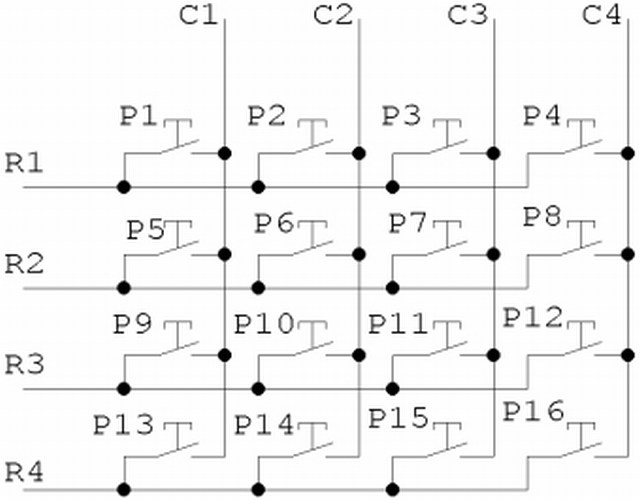
\includegraphics[width=0.35\linewidth]{img/pic_schema_tastiera.jpg}
\end{center}
\vspace*{0.25cm}

\noindent
To read the button pressed the rows must be connected to \(0V\) or \(V_{cc}\) and the column have to be read following this sequence:

\begin{itemize}

    \item \(R1 = V_{cc} \quad R2 = 0V \quad R3 = 0V \quad R4 = 0V\) \\
    the first row is enabled and the others are disabled, so the \(C_1 \quad ... \quad C4\) read values are referred to \(P1 \quad ...\quad P4\)

    \item \(R1 = 0V \quad R2 = V_{cc} \quad R3 = 0V \quad R4 = 0V\) \\
    the second row is enabled and the others are disabled, so the \(C_1 \quad ... \quad C4\) read values are referred to \(P5 \quad ...\quad P6\)
    
    \item \(R1 = 0V \quad R2 = 0V \quad R3 = V_{cc} \quad R4 = 0V\) \\
    the third row is enabled and the others are disabled, so the \(C_1 \quad ... \quad C4\) read values are referred to \(P9 \quad ...\quad P10\)
    
    \item \(R1 = 0V \quad R2 = 0V \quad R3 = 0V \quad R4 = V_{cc}\) \\
    the fourth row is enabled and the others are disabled, so the \(C_1 \quad ... \quad C4\) read values are referred to \(P13 \quad ...\quad P16\)
\end{itemize}

\noindent
Thus, the principle is to enable the row containing the pressed button and read the corresponding column wire. \\
The entire enable sequence (from enabling the first row to enabling the last row) must be completed faster than the user's response time. \\
This is usually not a problem, because a person has a response time greater than \(100 \, \mathrm{ms}\); therefore, with a scanning frequency greater than \(40 \, \mathrm{Hz} \simeq \text{row\_number}/100\,\mathrm{ms}\), the user does not perceive any delay when pressing the button.
To read the keypad, the rows must be enabled sequentially. \\
However, if two buttons in the same column are pressed at the same time, the rows can become shorted, which may be dangerous for the system. \\
For this reason, diodes are used when connecting the rows. \\
The columns are floating when no button is pressed, so pull-down (or pull-up, depending on the keypad reading logic) resistors are required.


\newpage

\subsection{LCD communication}

We use the \textbf{16x2 LCD Module} (\texttt{CFAH1602B-TMC-JP}) integrated in the \textbf{Altera DE2 board} to show the selected wave function name and wave frequency. \\
The LCD Module has built in a LSI controller, the controller has two 8-bit registers, an \textbf{instruction register} (IR) and a \textbf{data register} (DR). \\
The IR stores instruction codes, such as display clear and cursor shift, and address information for display data RAM (DDRAM). \\
These two registers can be selected with the \textbf{register selector} (RS) signal, if it is set to low is possible to write an operation into the IR register, else if the RS signal is set to high the data are written from the DR to the DDRAM. \\
The R/W pin can be used to read the Busy Flag (BF), if is enabled, or to read data from DDRAM or CGRAM. \\
Since we don't need those functions we leave it always low.

\vspace{0.5cm}
\begin{figure}[h!]
    \centering
    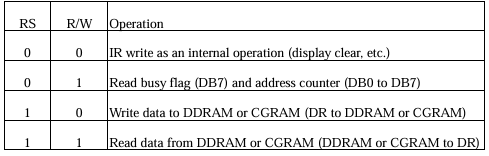
\includegraphics[width=0.6\linewidth]{img/LCD_rs_rw_table.png}
    \caption{Operation selection}
    \label{fig:LCD_rs_rw_table}
\end{figure}
\vspace{0.5cm}

\subsubsection{Character display}
An internal Address Counter (AC) is used to increment the DDRAM address each new writing cycle. \\
The Character Generator ROM (CGROM) generates 5x8 dot or 5x10 dot character patters from 8 bit ASCII code stored in the DDRAM to be displayed on the screen. \\
The table \autoref{fig:LCD_character_generator} shows how CGROM can output a unique set of dots for each character. 

\vspace{0.5cm}
\begin{figure}[h!]
    \centering
    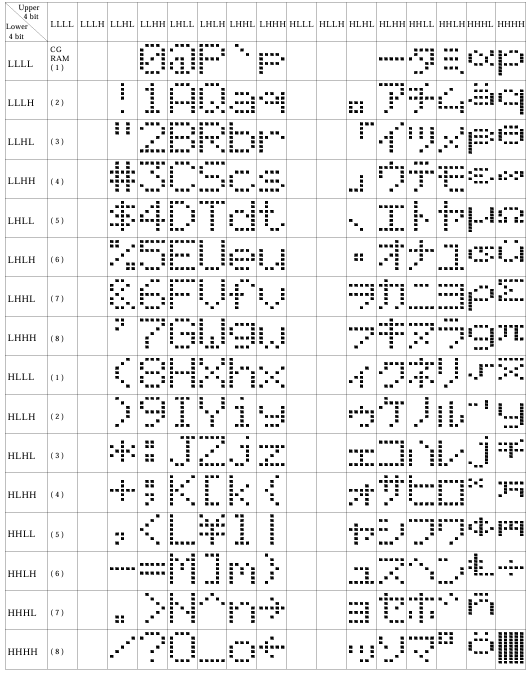
\includegraphics[width=0.45\linewidth]{img/LCD_character_generator.png}
    \caption{Character Generator ROM pattern}
    \label{fig:LCD_character_generator}
\end{figure}
\vspace{0.5cm}

\subsubsection{Timing Characteristics}
It is essential to respect the timing characteristic of LCD module to correctly complete a write cycle without issues. \\
As we can see in \autoref{fig:LCD_write_cycle} the RS and R/W signals need to be stable before the E signal is set to high and the enable pulse needs to be sufficiently wide to collect the data, then after disabling E an hold time is required to complete the cycle. \\
In our case a fast display refresh frequency is not required, so it is possible to use delays way larger than the stated times reported by the datasheet, nonetheless the correct sequence of the chip enable (E) needs to be used.

\vspace{0.5cm}
\begin{figure}[h!]
    \centering
    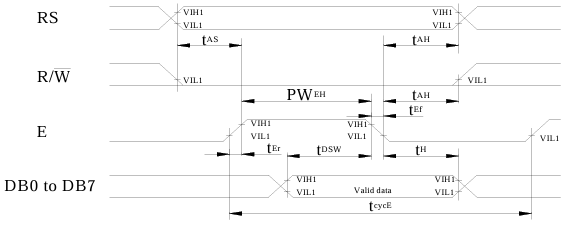
\includegraphics[width=0.8\linewidth]{img/LCD_write_cycle.png}
    \caption{Write Operation}
    \label{fig:LCD_write_cycle}
\end{figure}
\vspace{0.5cm}